\chapter{Das Photon in der Quantenelektrodynamik (QED)}\index{Photon}\index{Quantenelektrodynamik (QED)}
\setcounter{section}{5}
\setcounter{subsection}{0}
\setcounter{subsubsection}{1}
\setcounter{secnumdepth}{3}
\setlength{\parindent}{0pt}
% Boxen-Stile definieren
\tcbset{physikbox/.style={colback=blue!5!white, colframe=blue!75!black, fonttitle=\bfseries}}
\tcbset{mathebox/.style={colback=green!5!white, colframe=green!50!black, fonttitle=\bfseries}}
\tcbset{didaktikbox/.style={colback=yellow!5!white, colframe=yellow!50!black, fonttitle=\bfseries}}
\tcbset{hypobox/.style={colback=orange!5!white, colframe=orange!75!black, fonttitle=\bfseries}}
\tcbset{hinweisbox/.style={colback=gray!10!white, colframe=black!40!black, fonttitle=\bfseries}}
\tcbset{warnbox/.style={colback=red!10!white, colframe=red!40!black, fonttitle=\bfseries}}

\subsection{Vom Photon zur Quantenelektrodynamik}\index{Quantenelektrodynamik (QED)!Einführung}\index{Photoeffekt}\index{Compton-Streuung}\index{Einstein, Albert}\index{Maxwell, James Clerk}\index{Austauschteilchen}
% Historischer und theoretischer Übergang: von der klassischen Elektrodynamik über die Quantenoptik zur QED

Die Geschichte des Photons beginnt mit einem Paradoxon: Das Licht, das man seit dem 19. Jahrhundert als elektromagnetische Welle verstand, zeigte bei bestimmten Experimenten ein Verhalten, das nur mit einem Teilchenbild erklärbar war – insbesondere beim Photoeffekt und der Compton-Streuung.\index{Wellenmodell}\index{Teilchenmodell}
Diese Experimente führten zur Einführung des Begriffs des \emph{Lichtquants} durch Einstein im Jahr 1905.\index{Lichtquant}
Doch obwohl sich das Photonenmodell experimentell bewährte, blieb es über Jahrzehnte umstritten.\index{Photonenmodell}

Ein vollständiges theoretisches Verständnis der Lichtmaterie-Wechsel\-wirkung gelang erst mit der Entwicklung der \textbf{Quantenelektrodynamik} (QED).\index{Licht-Materie-Wechsel wirkung}\index{Relativitätstheorie!Spezielle}\index{Quantenmechanik}
Sie verbindet die klassische Feldtheorie Maxwells mit den Prinzipien der Quantenmechanik und der speziellen Relativitätstheorie.
In der QED ist das Photon das Austauschteilchen der elektromagnetischen Wechselwirkung – ein masseloses, Spin-1-Trägerteilchen, das nicht nur reale, sondern auch virtuelle Zustände annehmen kann.\index{Spin}\index{Masselosigkeit}\index{Virtuelle Photonen}
(Eine kompakte Einführung in den Feldformalismus der QED und das Potential \(A^\mu\) findet sich in Anhang~A, Abschnitt~\ref{anhangA:feldformalismus}.)

\medskip
\begin{tcolorbox}[physikbox, title=Was ist Quantenelektrodynamik?]
	\label{box:was ist quantenelektro}
	\small
	Die Quantenelektrodynamik beschreibt, wie geladene Teilchen (z.\,B. Elektronen) Photonen austauschen und dadurch elektromagnetisch miteinander wechselwirken.\\
	Die Theorie basiert auf quantisierten Feldern, Feynman-Diagrammen und einem lokalen Eichprinzip. Sie ist die präziseste physikalische Theorie, die bisher experimentell getestet wurde.
\end{tcolorbox}
\medskip
Der Übergang vom klassischen zum quantenfeldtheoretischen Verständnis war jedoch alles andere als geradlinig. Anfangs betrachtete man Photonen als diskrete Pakete klassischer Wellenenergie – ein Kompromiss zwischen Teilchen- und Wellenbild.\index{Quantenfeldtheorie}\index{Wellenenergie}
Erst in den 1940er-Jahren, mit der Arbeit von Dirac, Feynman, Schwinger und Tomonaga, entstand eine konsistente Theorie, die das Photon als Quant des elektromagnetischen Feldes mathematisch beschreibt.\index{Dirac, Paul A. M.}\index{Feynman, Richard P.}\index{Schwinger, Julian}\index{Tomonaga, Sin-Itiro}\index{Quantisiertes Feld}

\textbf{Was sich mit QED ändert:}
\begin{itemize}
	\item Photonen werden nicht mehr als Lichtstrahlen gedacht, sondern als Anregungen eines quantisierten Feldes.\index{Anregung (Feld)}\index{Lichtstrahl}
	\item Die Wechselwirkung erfolgt nicht kontinuierlich, sondern in diskreten Prozessen (Vertices).\index{Wechselwirkung!Vertex}
	\item Auch virtuelle Photonen – nicht beobachtbar, aber mathematisch erforderlich – spielen eine zentrale Rolle.\index{Virtuelle Photonen}
\end{itemize}
(Zum Übergang vom klassischen Feld zur Quantisierung und zu Feynman-Diagrammen vgl. Anhang~A, Abschnitt~\ref{anhangA:feld_zu_qed}.)

Dieses Kapitel führt in die Eigenschaften des Photons im Rahmen der QED ein, beginnend mit seinem Vektorcharakter, gefolgt von seiner Rolle als Austauschteilchen in Feynman-Diagrammen, bis hin zu experimentellen Bestätigungen mit höchster Präzision.\index{Feynman-Diagramme}

\subsection{Der Vektorcharakter des Photons in der QED}\index{Photon!Vektorcharakter}\index{Polarisation!Transversal}\index{Spin}

Die transversale Polarisation des Photons und seine Eigenschaft als Spin\mbox{-}1\mbox{-}Teilchen wurden bereits in Abschnitt~3.6 beschrieben.\index{Helizität}
In der Quantenelektrodynamik ergibt sich diese Struktur jedoch nicht nur aus experimenteller Beobachtung oder klassischen Gleichungen, sondern aus dem zugrunde liegenden \emph{Feldformalismus} und der \emph{Eichsymmetrie} der Theorie.\index{Feldformalismus}\index{Eichsymmetrie}
(Eine formale Darstellung der Helizität des Photons findet sich zusätzlich in Anhang~A, Abschnitt~\ref{anhangA:helizitaet}; zur Polarisation in Jones-/Dirac-Notation siehe \ref{anhangA:polarisation}.)

\medskip
\begin{tcolorbox}[physikbox, title=Was ist der Feldformalismus?]
	\label{box:was ist Feldformalismus}
	\small
	In der QED sind Photonen keine „Teilchen mit Bahn“, sondern quantisierte Anregungen eines Feldes: des elektromagnetischen Potentials \( A^\mu(x) \). So wie eine Wasserwelle ein lokaler Ausschlag der Wasseroberfläche ist, ist ein Photon eine diskrete Schwingung des Feldes – beschrieben durch Quantenmechanik und Relativität zugleich.
\end{tcolorbox}
\medskip
\index{Vektorpotential $A^\mu$}
(Eine kurze Ableitung der Lorentz-kovarianten Form des Viererpotentials \(A^\mu\) steht in Anhang~A, Abschnitt~\ref{anhangA:viererpotential}.)

Der zentrale mathematische Ausgangspunkt ist die sogenannte \emph{Lagrangedichte} \( \mathcal{L} \), aus der die Bewegungsgleichungen des Feldes abgeleitet werden.\index{Lagrangedichte}\index{Bewegungsgleichungen}
Für das elektromagnetische Feld lautet sie:

\[
\mathcal{L}_{\text{EM}} = -\frac{1}{4} F_{\mu\nu} F^{\mu\nu}
\quad \text{mit} \quad F_{\mu\nu} = \partial_\mu A_\nu - \partial_\nu A_\mu
\]\index{Feldstärketensor $F_{\mu\nu}$}
(Herleitung von Feldstärketensor und EM-Lagrangedichte: Anhang~A, Abschnitte~\ref{anhangA:feldstaerketensor} und \ref{anhangA:lagrange_em}; zur Energie-Impuls-Relation vgl. \ref{anhangA:energie_impuls}.)

Diese Lagrangedichte führt – über das Prinzip der kleinsten Wirkung – auf die Maxwellschen Gleichungen in ihrer relativistischen Form.\index{Prinzip der kleinsten Wirkung}\index{Maxwellsche Gleichungen}
Sie ist invariant unter sogenannten \textbf{Eichtransformationen}:

\[
A^\mu(x) \rightarrow A^\mu(x) + \partial^\mu \Lambda(x)
\]\index{Eichtransformation}
(Zur lokalen \(U(1)\)-Eichsymmetrie, Eichfixierung und  Lorenz-Bedingung siehe Anhang~A, Abschnitt~\ref{anhangA:eichsymmetrie}.)
\medskip
\begin{tcolorbox}[physikbox, title=Was bedeutet Eichsymmetrie?]
	\label{box:was bedeutet Eichsy}
	\small
	Eichsymmetrie bedeutet, dass man das elektromagnetische Potential \( A^\mu(x) \) lokal verändern kann, ohne dass sich messbare Größen wie das elektrische Feld ändern. Diese Freiheit ist kein Rechenkunststück, sondern strukturbildend: Sie bestimmt, welche Terme erlaubt sind – und welche nicht.
\end{tcolorbox}

\textbf{Warum ist das Photon masselos?}\index{Masselosigkeit}
Ein Masseterm der Form \( \frac{1}{2} m^2 A_\mu A^\mu \) wäre unter dieser Transformation \emph{nicht invariant}. Die Forderung nach Eichsymmetrie verbietet ihn – das Photon muss masselos sein.\index{Masseterm}\index{Eichinvarianz}
(Formale Argumentation via Proca-Lagrange­dichte und gebrochene Eichinvarianz: Anhang~A, Abschnitt~\ref{anhangA:masselosigkeit_proca}.)

\textbf{Warum ist das Photon transversal?}\index{Transversalität}
Ein Vektorfeld hat vier Komponenten, aber nicht alle sind physikalisch unabhängig. Die Eichfreiheit und die Lorentz-Invarianz erlauben es, nicht-physikalische Moden zu eliminieren. Am Ende bleiben genau zwei zulässige Polarisationszustände: die transversalen mit Helizität \( +1 \) und \( -1 \).\index{Lorentz-Invarianz}\index{Polarisationszustände}
(Reduktion der Freiheitsgrade, Lorenz-Bedingung und Spur/Projektor-Methode: Anhang~A, Abschnitt~\ref{anhangA:transversalitaet}; vgl. auch \ref{anhangA:helizitaet}.)

\medskip
\begin{tcolorbox}[physikbox, title=Folgen der Eichsymmetrie]
	\label{box:folgen der Eichsy}
	\small
	Die Eichsymmetrie der QED erklärt zwei grundlegende Eigenschaften des Photons:
	
	\begin{itemize}
		\item \textbf{Masselosigkeit:} Ein Masseterm wäre nicht eichinvariant – daher ist das Photon zwingend masselos.
		\item \textbf{Transversalität:} Die Symmetrie erlaubt nur zwei Polarisationsmoden – beide senkrecht zur Ausbreitungsrichtung.
	\end{itemize}
\end{tcolorbox}

\textbf{Virtuelle Photonen – eine Ausnahme}\index{Virtuelle Photonen}
Während reale Photonen ausschließlich transversale Zustände besitzen, können sogenannte \emph{virtuelle Photonen} – die in inneren Linien von Feynman-Diagrammen auftreten – auch longitudinale oder skalare Komponenten enthalten.\index{Longitudinale Mode}\index{Skalare Mode}
Diese sind jedoch nicht beobachtbar und verschwinden bei physikalischen Vorhersagen (z.\,B. in der Streuamplitude) vollständig.\index{Streuamplitude}
(Longitudinale/skalarer Anteile in Propagatoren und ihre Auslöschung in Observablen: Anhang~A, Abschnitt~\ref{anhangA:virtuelle_moden}.)

\textbf{Fazit:}\index{Eichsymmetrie!Folgen}
In der QED ergibt sich die Struktur des Photons nicht durch Zusatzannahmen, sondern aus dem symmetrischen Aufbau der Theorie selbst. Die Eichsymmetrie ersetzt Intuition – und erzeugt Ordnung.

%index Anhang
\subsection{Virtuelle Photonen und Feynman-Diagramme}\index{Virtuelle Photonen}\index{Feynman-Diagramme}

\subsubsection{Was sind virtuelle Teilchen?}\index{Virtuelle Teilchen}
\addcontentsline{toc}{subsubsection}{5.3.1 Was sind virtuelle Teilchen?}

Virtuelle Teilchen – insbesondere virtuelle Photonen – sind zentrale Rechenelemente in der Quantenfeldtheorie.\index{Quantenfeldtheorie}
Sie unterscheiden sich grundlegend von realen Teilchen, wie sie in einem Detektor nachgewiesen werden können.\index{Reale Teilchen}\index{Detektor}
Ihre Existenz ist \textbf{mathematischer Natur} – und dennoch zeigen sich ihre Wirkungen in realen Experimenten.\index{Mathematisches Objekt}

\subsubsection*{Unterschied: reale  oder virtuelle Teilchen}\index{On-shell}\index{Off-shell}
\phantomsection
\begin{table}[H]
	\centering
	\scriptsize 

{\small
	\begin{center}
		\renewcommand{\arraystretch}{1.3}
		\begin{tabular}{|p{3cm}|p{3.0cm}|p{3.0cm}|}
			\hline
			\textbf{Eigenschaft} & \textbf{Reale Photonen} & \textbf{Virtuelle Photonen} \\
			\hline
			Beobachtbar im Detektor & Ja (z.\,B. Lichtquant im Photoeffekt) & Nein \\
			\hline
			Energie-Impuls-Beziehung & $E = pc$ (on-shell) & $E^2 \ne p^2 c^2$ (off-shell) \\
			\hline
			Lebensdauer & Beliebig lang (bei stabilen Teilchen) & Extrem kurz (durch Unschärferelation) \\
			\hline
			Physikalische Existenz & Ja & Nur als Rechenelement in Diagrammen \\
			\hline
		\end{tabular}
	\end{center}
}
\end{table}
\medskip

% Mathebox: On-shell-Bedingung
\begin{tcolorbox}[hinweisbox, title=On-shell-Bedingung]
	\label{box:On-shell-Bedingung}
	Ein Teilchen ist \textbf{on-shell}, wenn es die relativistische Energie-Impuls-Beziehung erfüllt:
	\[
	E^2 = p^2 c^2 + m^2 c^4
	\]
	Für masselose Teilchen (z.\,B. Photonen) reduziert sich dies auf:
	\[
	E = pc
	\]
	Off-shell-Zustände treten bei virtuellen Teilchen auf, die nur in Zwischenrechnungen vorkommen.
\end{tcolorbox}
\index{Energie-Impuls-Beziehung}\index{Relativistische Kinematik}

\subsubsection*{Zeit-Energie-Unschärfe}\index{Unschärferelation!Zeit-Energie}
\phantomsection
Nach der Heisenbergschen Unschärferelation gilt:
\[
\Delta E \cdot \Delta t \gtrsim \hbar
\]\index{Heisenberg, Werner}\index{$\hbar$}
Für sehr kurze Zeiten $\Delta t$ ist es also möglich, kurzfristig gegen die Energieerhaltung zu „verstoßen“ – z.\,B. durch das Auftreten eines virtuellen Photons mit scheinbar „falscher“ Energie.\index{Energieerhaltung}
Dieser Effekt ist kein Regelbruch, sondern eine Konsequenz der Quantenmechanik.\index{Quantenmechanik}

\subsubsection*{Interpretation}\index{Zwischenzustand}
\phantomsection

Virtuelle Teilchen treten in \textbf{Zwischenzuständen} auf – etwa wenn ein Elektron kurz ein Photon abstrahlt, das sofort wieder absorbiert wird.\index{Elektron}\index{Absorption}\index{Emission}
Diese Prozesse finden in \textbf{Feynman-Diagrammen} ihren Ausdruck. Die virtuellen Teilchen sind dabei die \textbf{inneren Linien} des Diagramms.\index{Innere Linien (Diagramme)}

\medskip

% Physikbox: Virtuelle Teilchen

\medskip
\begin{tcolorbox}[physikbox, title=Virtuelle Teilchen im Quantenvakuum, label=box:virtuelle-teilchen]
	\label{box:virtuelle-teilchen}
	Virtuelle Teilchen entstehen als Zwischenzustände bei quantenmechanischen Wechselwirkungen. Sie erfüllen nicht die klassische Energie-Impuls-Beziehung (sind \emph{off-shell}) und können nicht direkt beobachtet werden.
	
	Trotzdem zeigen sich ihre Effekte in präzisesten Experimenten – etwa beim \textbf{Lamb-Shift} im Wasserstoffspektrum oder bei der \textbf{Anomalie des $g$-Faktors} des Elektrons.
\end{tcolorbox}
\index{Quantenvakuum}\index{Lamb-Shift}\index{g-Faktor!Anomalie}\index{Wasserstoffspektrum}

\medskip
\begin{tcolorbox}[hinweisbox, title=Indirekte Nachweise virtueller Photonen]
	\label{box:Nachweis virtueller Photonen}
	\small
	\begin{itemize}
		\item \textbf{Lamb-Shift:} In hochpräzisen Spektren des Wasserstoffatoms zeigt sich eine feine Verschiebung der Energieniveaus, die nur mit quantenfeldtheoretischen Korrekturen erklärt werden kann – insbesondere durch den Einfluss virtueller Photonen auf das Elektron.
		\item \textbf{$g$-Faktor-Anomalie:} Das Elektron besitzt ein magnetisches Moment, das geringfügig vom klassischen Wert $g = 2$ abweicht. Diese Abweichung entsteht durch Schleifenprozesse in Feynman-Diagrammen – mit virtuellen Photonen als Vermittlern.
	\end{itemize}
\end{tcolorbox}
\index{Schleifenprozesse}\index{Magnetisches Moment}\index{Elektron}

\medskip
% Didaktikbox: Denkfehler vermeiden
\begin{tcolorbox}[didaktikbox, title=Virtuell heißt nicht: weniger real?, label=box:virtuell-denkfehler]
	\label{box:virtuell-denkfehler}
	Der Begriff \glqq virtuell\grqq{} kann leicht in die Irre führen. Virtuelle Teilchen sind \textbf{nicht einfach „unreale“ Teilchen} – sie sind präzise definierte mathematische Objekte in der Quantenfeldtheorie.
	
	Sie folgen eigenen Regeln und tragen wesentlich zum richtigen Ergebnis bei – gerade weil sie \emph{nicht} die Bedingungen realer Teilchen erfüllen.
\end{tcolorbox}


\medskip

\subsubsection*{Übergang}\index{Coulomb-Kraft}\index{Streuung}
\phantomsection

Im nächsten Abschnitt betrachten wir, wie genau diese virtuellen Photonen in der Quantenfeldtheorie die elektromagnetische Wechselwirkung vermitteln – von der klassischen Coulomb-Kraft bis zu Streuprozessen.
\subsubsection{Virtuelle Photonen als Austauschteilchen}\index{Virtuelle Photonen!Austauschteilchen}\index{Austauschteilchen}\index{Wechselwirkung!elektromagnetisch}

In der klassischen Physik wird die elektromagnetische Kraft als ein Feld beschrieben, das von Ladungen erzeugt wird und auf andere Ladungen wirkt – wie im Coulomb-Gesetz\index{Coulomb-Gesetz} oder in Maxwells Gleichungen\index{Maxwellsche Gleichungen}. In der Quantenfeldtheorie hingegen wird die Kraftwirkung durch den Austausch von virtuellen Photonen vermittelt.\index{Virtuelle Photonen}

Diese virtuellen Photonen treten in Wechselwirkungsprozessen zwischen geladenen Teilchen auf, ohne dass sie als reale Lichtquanten nachgewiesen werden.\index{Reale Photonen} Sie sind nicht beobachtbar – und dennoch sind sie das zentrale Element, durch das sich Kräfte quantenmechanisch erklären lassen.\index{Kraft!quantenmechanische Vermittlung}

\subsubsection*{Austauschbild statt Kraftbild}\index{Austauschbild}\index{Kraftbild}\index{Impulsübertrag}
\phantomsection

Statt sich eine „Kraft“ im klassischen Sinn vorzustellen, denkt man sich in der QED, dass Teilchen sich gegenseitig \emph{virtuelle Photonen zusenden}, die den Impuls übertragen. Dadurch entsteht der Eindruck einer Wechselwirkung. \index{QED}\index{Wechselwirkung!Austauschprinzip}
\medskip
\begin{tcolorbox}[physikbox, title=Virtuelle Photonen als Kraftvermittler]
	\label{box:Virtuelle Photonen als kraftvermittler}
	Virtuelle Photonen übertragen Impuls zwischen geladenen Teilchen und vermitteln so die elektromagnetische Wechselwirkung. Dieser Prozess ist die quantenfeldtheoretische Erklärung für Kräfte wie die Coulomb-Kraft oder den Magnetismus.
	
	Dabei „fliegt“ kein reales Photon zwischen den Teilchen – die Wirkung entsteht ausschließlich durch mathematisch beschriebene Zwischenzustände im Feynman-Diagramm.
\end{tcolorbox}
\index{Kraftvermittler}\index{Feynman-Diagramme}

\subsubsection*{Beispiel: Elektron-Elektron-Streuung}\index{Elektron-Elektron-Streuung}\index{Møller-Streuung}\index{Streuung!elastisch}
\phantomsection
Ein besonders anschauliches Beispiel ist die sogenannte \emph{Møller-Streuung}, bei der zwei Elektronen elastisch miteinander stoßen. In der klassischen Physik würde man von einer abstoßenden Coulomb-Kraft sprechen – in der QED jedoch beschreibt man den Prozess als Austausch eines virtuellen Photons zwischen den Elektronen.\index{Coulomb-Kraft}\index{Virtuelle Photonen!Austausch}
\begin{figure}[H]
	\begin{center}
		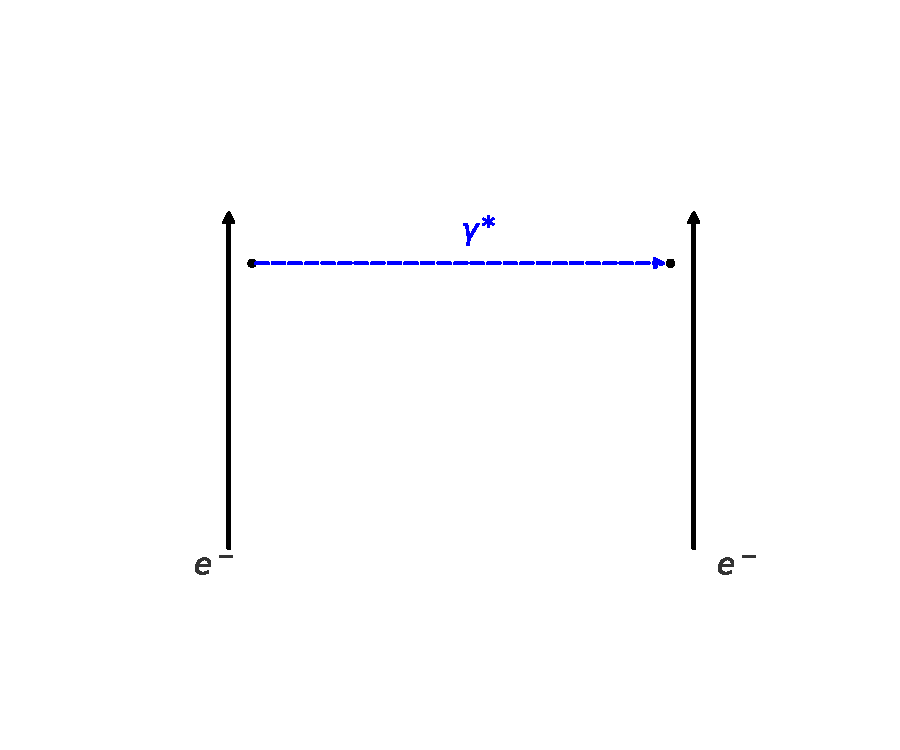
\includegraphics[width=0.4\linewidth]{bilder/moeller-diagramm.pdf}
	\end{center}
	\caption{Das virtuelle Photon ist hier die innere Linie des Feynman-Diagramms. Es vermittelt Impuls – obwohl es niemals real existiert.}
\end{figure}

\subsubsection*{Was zeigt dieses Diagramm?}\index{Feynman-Diagramme!Deutung}\index{Innere Linien (Diagramme)}\index{Vertex}\index{Impulsübertragung}\index{Energieübertragung}
\phantomsection
Das Feynman-Diagramm stellt eine typische \textbf{Møller-Streuung} dar – die elastische Streuung zweier Elektronen durch den Austausch eines virtuellen Photons. Die Zeitachse verläuft dabei von unten nach oben.\index{Zeitachse (Diagramm)}

\begin{itemize}
	\item \textbf{Zwei Elektronen} kommen von unten ins Bild (linke und rechte Seite). Sie bewegen sich aufeinander zu und treten in Wechselwirkung.\index{Elektron}
	
	\item Das \textbf{virtuelle Photon} (gekennzeichnet durch die gestrichelte blaue Linie und das Symbol $\gamma^*$) wird zwischen den Elektronen ausgetauscht.\index{Photon!virtuell $\gamma^*$} Es ist \emph{nicht real}, sondern ein Zwischenzustand der quantenfeldtheoretischen Rechnung.\index{Zwischenzustand}
	
	\item Das Photon überträgt Impuls und Energie – dadurch ändern die Elektronen ihre Bewegungsrichtung und verlassen das Wechselwirkungsgebiet gestreut nach oben.\index{Streuwinkel}
	
	\item Die beiden \textbf{Vertices} (Verbindungspunkte) zeigen, wo die Wechselwirkung lokalisiert ist. Dort findet mathematisch der Impulsübertrag statt.\index{Vertex}
\end{itemize}

\begin{tcolorbox}[didaktikbox, title=Was zeigt das Feynman-Diagramm wirklich?]
	\label{box:Was zeigt das Feynman-Diagramm wirklich}
	Das gezeigte Diagramm der Møller-Streuung zeigt nicht, wie ein reales Photon zwischen Elektronen fliegt. Vielmehr beschreibt es einen quantenmechanischen Übergangszustand:
	
	Ein \textbf{virtuelles Photon} vermittelt die Wechselwirkung – mathematisch im Rahmen der Störungsrechnung. Dieses Photon erfüllt nicht die klassische Beziehung $E = pc$, es existiert nur als \emph{off-shell}-Zwischenzustand und überträgt Impuls.
	
	Reale Effekte wie Streuwinkel und Energieverteilung lassen sich daraus berechnen – ohne dass je ein Photon detektiert wird.
\end{tcolorbox}
\index{Störungsrechnung}\index{Off-shell}\index{Energieverteilung}

\subsubsection*{Keine direkte Beobachtbarkeit – aber messbare Wirkung}\index{Wirkungsquerschnitt}\index{Messgrößen}
\phantomsection
Virtuelle Photonen sind nicht detektierbar. Dennoch beeinflussen sie messbare Größen: Wirkungsquerschnitte, Streuwinkel und Energieverteilungen lassen sich mit hoher Genauigkeit durch die zugrunde liegende Austauschart beschreiben.

\subsubsection*{Abgrenzung zur realen Photonenerzeugung}\index{Compton-Effekt}\index{Photonenprozesse}\index{Austauschdiagramme}\index{Reale Photonen}
\phantomsection
Ein wichtiger Unterschied: Beim \emph{Compton-Effekt} wird ein \textbf{reales} Photon gestreut – mit Nachweis im Detektor. Beim \textbf{virtuellen Austausch} hingegen ist kein Photon als reales Teilchen beteiligt. Das ist der fundamentale Unterschied zwischen \textbf{Austauschdiagrammen} und \textbf{Photonenprozessen}.

\medskip

% Didaktikbox: Kein klassisches Kraftfeld
\begin{tcolorbox}[didaktikbox, title=Keine „unsichtbare Kraft“ mehr nötig]
	\label{box:unsichtbare Kraft}
	In der Quantenfeldtheorie braucht man kein klassisches Kraftfeld mehr, das zwischen zwei Ladungen wirkt. Stattdessen entstehen Wechselwirkungen durch den Austausch von virtuellen Teilchen – hier: virtuellen Photonen.
	
	Das klassische Bild der Fernwirkung wird so durch ein lokales, quantisiertes Austauschprinzip ersetzt.
\end{tcolorbox}
\index{Fernwirkung}\index{Lokalität}\index{Austauschprinzip}

\subsubsection{Feynman-Diagramme als visuelle Rechenhilfe}\index{Feynman-Diagramme!Rechenhilfe}\index{Wahrscheinlichkeitsamplitude}\index{Störungsrechnung}

Die sogenannten \textbf{Feynman-Diagramme} sind ein zentrales Werkzeug der Quantenfeldtheorie – insbesondere in der Quantenelektrodynamik (QED).\index{Quantenfeldtheorie}\index{QED} Sie dienen als \emph{grafische Notation} für mathematische Terme in der Störungsrechnung und helfen dabei, komplexe Prozesse anschaulich zu strukturieren.

Ein Diagramm stellt keinen realen „Ablauf in Raum und Zeit“ dar, sondern kodiert eine Wahrscheinlichkeitsamplitude. Dennoch lassen sich daraus physikalisch messbare Größen wie Streuwinkel, Wirkungsquerschnitte oder Lebensdauern berechnen.\index{Lebensdauer}

\subsubsection*{Elemente eines Feynman-Diagramms}\index{Fermionlinien}\index{Photonenlinien}\index{Vertices}\index{Zeitachse (Diagramm)}
\phantomsection
\begin{itemize}
	\item \textbf{Fermionlinien:} durchgezogene Linien mit Pfeil – z.\,B. Elektronen oder Positronen
	\item \textbf{Photonenlinien:} wellige oder gestrichelte Linien – je nach Konvention
	\item \textbf{Vertices:} Punkte, an denen Teilchen „wechselwirken“, also Impuls übertragen wird
	\item \textbf{Zeitachse:} meist von unten nach oben oder von links nach rechts
\end{itemize}
\begin{figure}[H]
	\begin{center}
		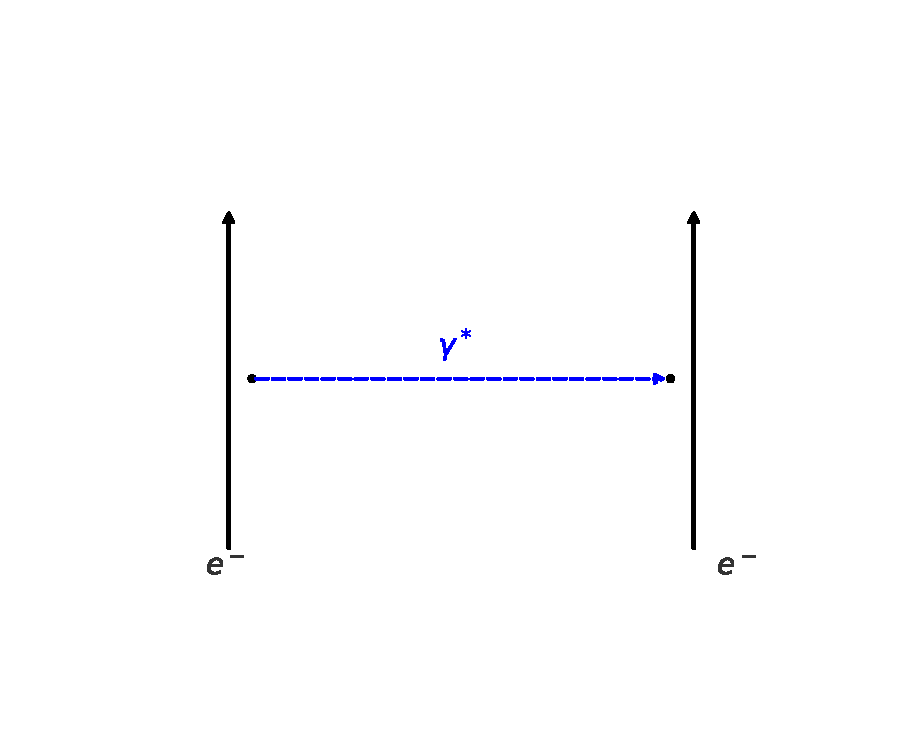
\includegraphics[width=0.45\linewidth]{bilder/feynman-einphoton.pdf}
	\end{center}
	\caption{Feynman-Diagramm}
\end{figure}

\vspace{0.5em}
\begin{tcolorbox}[physikbox, title=Was ein Feynman-Diagramm wirklich zeigt]
	\label{box:Was ein Feynman-Diagramm}
	Ein Feynman-Diagramm ist kein klassischer Bewegungsfilm, sondern eine symbolische Darstellung eines mathematischen Integrals über alle möglichen Pfade eines Prozesses. Es kodiert die Struktur der Wahrscheinlichkeitsamplitude, nicht die exakte Bahn einzelner Teilchen.
\end{tcolorbox}
\index{Pfadintegral}

\subsubsection*{Beispiel: Ein-Photon-Austausch}\index{Ein-Photon-Austausch}\index{Elektron-Elektron-Streuung}\index{Impulsübertrag}
\phantomsection
Beim elastischen Elektron-Elektron-Stoß besteht das zugehörige Feyn\-man-Diagramm aus zwei einlaufenden und zwei auslaufenden Elektronenlinien sowie einer virtuellen Photonenlinie dazwischen. Dieses Diagramm steht symbolisch für eine Formel, die über alle möglichen Impulsüberträge und Zeitpunkte summiert – es ersetzt nicht die Realität, sondern bildet sie probabilistisch ab.\index{Probabilistische Beschreibung}

\subsubsection*{Mehr als nur Bilder – Diagrammregeln}
\phantomsection
\index{Feynman-Regeln}\index{Propagator}\index{Kopplungskonstante}\index{Ladung!elektrische}\index{Amplitude!Streuamplitude}
Jedes Feynman-Diagramm entspricht einem mathematischen Ausdruck. Die sogenannte \emph{Feynman-Regel} weist z.\,B. jeder Linie einen Bruchterm (Propagator), jedem Vertex eine Kopplungskonstante (z.\,B. $e$), und dem Gesamtdiagramm ein Integral über Impulse zu. Die Summe aller möglichen Diagramme bis zu einem bestimmten Ordnungsniveau ergibt die physikalisch messbare Größe.\index{Impulsraum-Integral}\index{Ordnung (Störungstheorie)}

\medskip
\begin{tcolorbox}[didaktikbox, title=Diagramm ist nicht gleich Realität]
	\label{boxx:Diagramm ist nicht gleich realität}
	Ein häufiges Missverständnis ist, dass ein Feynman-Diagramm einen realen Ablauf zeigt – etwa wie ein Photon „fliegt“. Tatsächlich beschreibt es eine \emph{Überlagerung aller möglichen Zwischenzustände}, zusammengefasst in einer quantenmechanischen Amplitude. Es ist also ein Werkzeug des Rechnens, kein Film des Geschehens.
\end{tcolorbox}
\index{Überlagerung}\index{Zwischenzustand}

\subsubsection{Beispielhafte Diagramme}\index{Prozesse!QED}\index{Virtuelle Photonen!vs.\ reale Photonen}\index{Reale Photonen}
\phantomsection

Um die Rolle virtueller Photonen im Vergleich zu realen Photonen besser zu verstehen, lohnt sich ein Blick auf typische Prozesse in der Quantenelektrodynamik. Feynman-Diagramme zeigen dabei deutlich, ob ein Photon real (detektierbar) oder nur virtuell (vermittelt Wechselwirkung) ist.

\subsubsection*{1. Virtueller Austausch: Møller-Streuung (Elastischer $e^-e^-$-Stoß)}\index{Møller-Streuung}\index{Streuung!elastisch}\index{Virtuelle Photonen!Austausch}
\phantomsection
In diesem Prozess stoßen zwei Elektronen über den Austausch eines virtuellen Photons elastisch aneinander. Das Photon ist nicht real – es vermittelt lediglich Impuls.\index{Impulsübertragung}
\begin{figure}[H]
	\begin{center}
		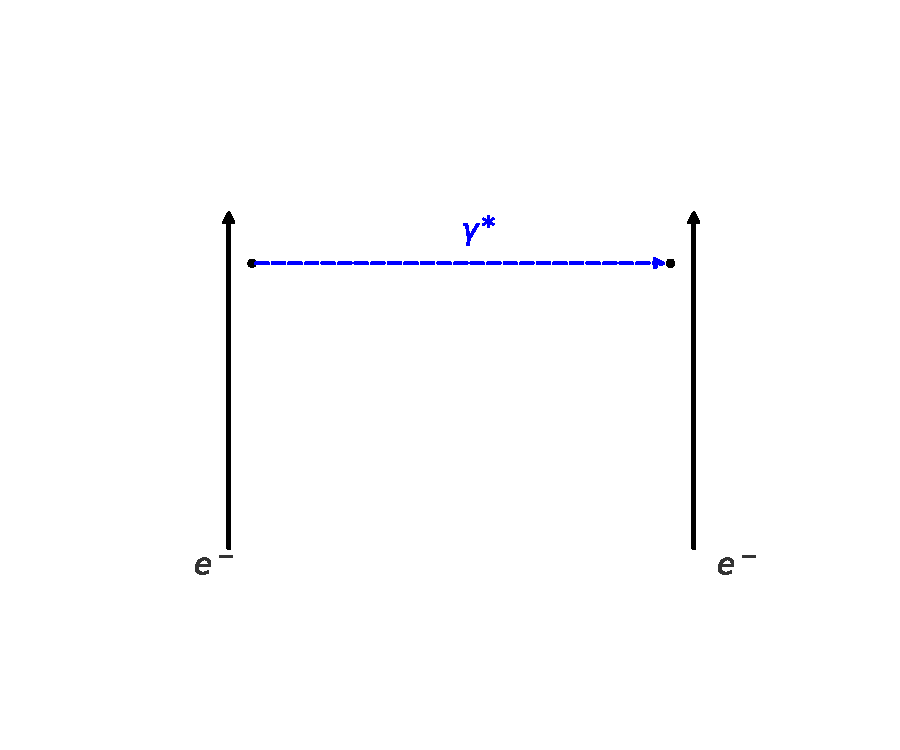
\includegraphics[width=0.42\linewidth]{bilder/moeller-diagramm.pdf}
	\end{center}
	\caption{Virtuelles Photon}
\end{figure}


\begin{tcolorbox}[physikbox, title=Virtuelles Photon]
	\label{box:virtuelles Photon}
	Das ausgetauschte Photon ist virtuell – es existiert nicht als reales Teilchen. Es überträgt Impuls und Energie, erfüllt aber nicht $E = pc$.
\end{tcolorbox}
\index{Photon!virtuell}\index{Energieübertragung}
\subsubsection*{2. Reales Photon: Compton-Streuung}\index{Compton-Effekt}\index{Reale Photonen}\index{Feynman-Diagramme!Compton-Streuung}\index{On-shell}\index{Elektronen-Propagator}\index{Vertex}
\phantomsection
Beim Compton-Effekt wird ein reales Photon an einem Elektron gestreut. Sowohl Ein- als auch Aus-Photon sind reale, detektierbare Teilchen.\index{Detektion} Das Feynman-Diagramm zeigt zwei Vertices mit einem internen Elektronen-Propagator.\index{Propagator!Elektron}\index{Vertices}

\begin{figure}[H]
	\begin{center}
		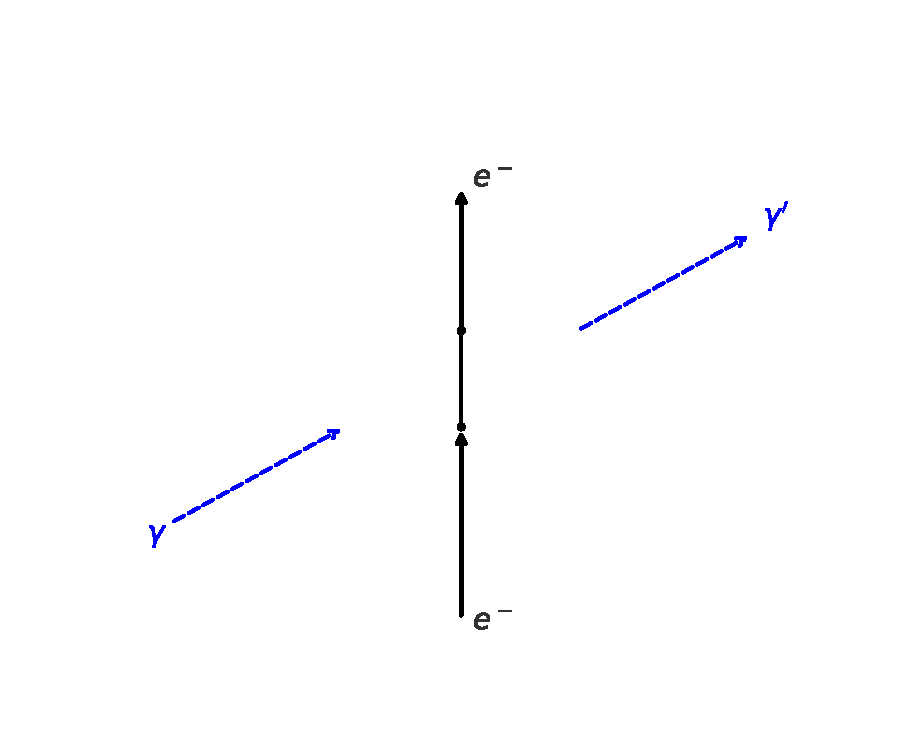
\includegraphics[width=0.5\linewidth]{bilder/compton-diagramm.pdf}
	\end{center}
	\caption{Reales Photon}
\end{figure}

\begin{tcolorbox}[physikbox, title=Reale Photonen]
	\label{box:Reale Photonen}
	In der Compton-Streuung treten Photonen als reale Teilchen auf. Sie sind messbar und erfüllen die on-shell-Bedingung $E = pc$.
\end{tcolorbox}
\index{Photon!real}\index{On-shell-Bedingung}

\subsubsection*{3. Schleifendiagramme: Selbstwechselwirkung und g-Faktor}\index{Schleifendiagramme}\index{Selbstenergie}\index{Vertexkorrektur}\index{g-Faktor!Anomalie}
\phantomsection
In höheren Ordnungen der Störungsrechnung tauchen geschlossene Schleifen in Feynman-Diagrammen auf – etwa bei der Selbstwechselwirkung eines Elektrons mit sich selbst über ein virtuelles Photon.\index{Virtuelle Photonen} Solche Diagramme erklären u.\,a. die Anomalie des $g$-Faktors.\index{Anomalie!$g$-Faktor}
\begin{figure}[H]
	\begin{center}
		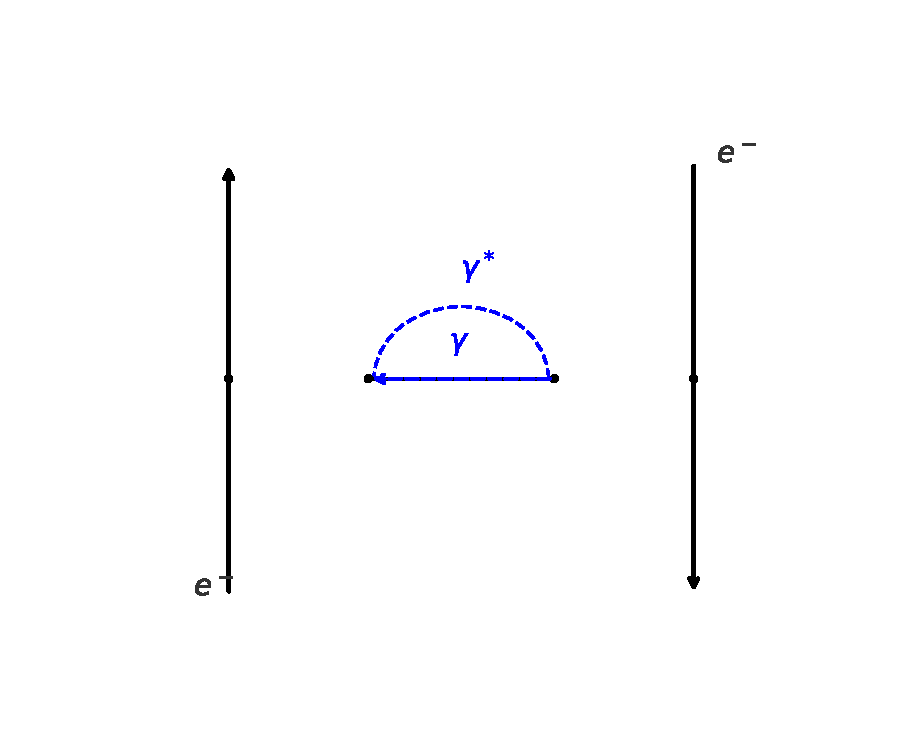
\includegraphics[width=0.4\linewidth]{bilder/vertex-korrektur.pdf}
	\end{center}
	\caption{Schleifendiagramm}
\end{figure}

\begin{tcolorbox}[hinweisbox, title=Schleifendiagramme und Präzisionseffekte]
	\label{box:Schleifendiagramme}
	Schleifen mit virtuellen Photonen liefern Korrekturen zu einfachen Prozessen – etwa für den exakten Wert des Elektron-$g$-Faktors oder den Lamb-Shift. Diese Effekte wurden experimentell mit hoher Präzision bestätigt.
\end{tcolorbox}
\index{Lamb-Shift}\index{Präzisionsexperimente}

\subsubsection*{Didaktischer Vergleich}\index{Didaktischer Vergleich}\index{Photonen!real vs.\ virtuell}
\phantomsection
\begin{itemize}
	\item \textbf{Virtuelle Photonen} treten als innere Linien in Diagrammen auf. Sie sind nicht direkt nachweisbar, aber physikalisch wirksam.\index{Innere Linien}\index{Nachweis!indirekt}
	\item \textbf{Reale Photonen} sind äußere Linien. Sie können gemessen werden und sind on-shell.\index{Äußere Linien}
\end{itemize}

\begin{tcolorbox}[didaktikbox, title=Reale oder virtuelle Photonen im Diagramm]
	\label{box:Reale oder virtuelle Photonen}
	Ob ein Photon real oder virtuell ist, erkennt man daran, ob es als ein- oder auslaufendes Teilchen dargestellt wird. Nur reale Photonen sind beobachtbar. Virtuelle Photonen sind innere Linien – sie „existieren“ nur innerhalb des Rechenwegs.
\end{tcolorbox}
\index{Beobachtbarkeit}\index{Einlaufende Teilchen}\index{Auslaufende Teilchen}

\subsubsection{Bedeutung für die QED}\index{QED!Bedeutung}\index{Elektromagnetische Wechselwirkung}

Die Quantenelektrodynamik (QED) ist die am genauesten bestätigte Theorie der Physik. Ihre enorme Präzision wäre ohne das Konzept der virtuellen Photonen und die Feynman-Diagramme nicht denkbar.\index{Feynman-Diagramme}\index{Virtuelle Photonen}

\subsubsection*{Zentrale Rolle der virtuellen Photonen}\index{Virtuelle Photonen!zentrale Rolle}\index{Störungsrechnung}
\phantomsection
Virtuelle Photonen ermöglichen die Berechnung der elektromagnetischen Wechselwirkung zwischen geladenen Teilchen auf quantenmechanischer Ebene. Sie treten in allen Ordnungen der Störungsrechnung auf – vom einfachen Austausch bis zu komplexen Schleifenprozessen.\index{Austauschprozesse}\index{Loop-Korrekturen}

\medskip
\begin{tcolorbox}[physikbox, title=Ohne virtuelle Photonen keine QED]
	\label{box:Ohne virtuelle Photonen keine}
	Virtuelle Photonen sind das Fundament der quantenfeldtheoretischen Beschreibung elektromagnetischer Prozesse. Ohne sie könnte die QED keine Kräfte vermitteln und keine quantitativen Vorhersagen machen.
\end{tcolorbox}

\subsubsection*{Feynman-Diagramme als methodisches Rückgrat}\index{Feynman-Diagramme!Methode}\index{Amplituden!Wahrscheinlichkeits-}
\phantomsection
Feynman-Diagramme liefern nicht nur eine anschauliche Darstellung, sondern auch eine präzise Rechenvorschrift. Für jede mögliche Wechselwirkung können alle erlaubten Diagramme gezeichnet und in einen mathematischen Ausdruck übersetzt werden. Die Summe aller Diagramme liefert die beobachtbare Amplitude.\index{Summe über Diagramme}

\subsubsection*{Beispiel: Berechnung des $g$-Faktors}\index{g-Faktor!Elektron}\index{Anomalous magnetic moment}
\phantomsection
Die Abweichung des gyromagnetischen Faktors des Elektrons vom klassischen Wert $g = 2$ ist eines der genauesten Experimente der modernen Physik. Die Korrektur ergibt sich aus einem Schleifenprozess mit einem virtuellen Photon – also aus einem Feynman-Diagramm zweiter Ordnung.\index{Zweite Ordnung}

\subsubsection*{Exaktheit der Theorie}\index{QED!Exaktheit}\index{Vergleich Theorie–Experiment}
\phantomsection
Die theoretisch berechneten Werte für Größen wie den Lamb-Shift, den Elektron-$g$-Faktor oder Streuwinkel in Elektron-Stößen stimmen mit den Messergebnissen auf viele Dezimalstellen überein.\index{Streuwinkel}\index{Elektron-Streuung}
\medskip
\begin{tcolorbox}[didaktikbox, title=Die Quantenelektrodynamik als Erfolgsmodell]
	\label{box:Die Quantenelekrodynamik}
	Die QED ist nicht nur eine elegante Theorie – sie liefert mit Hilfe virtueller Teilchen und Feynman-Diagrammen quantitative Vorhersagen mit einer Genauigkeit von bis zu 12 Dezimalstellen. Die Rolle des Photons – auch als virtuelles Teilchen – steht dabei im Zentrum.
\end{tcolorbox}
\index{Erfolgsmodell}\index{Genauigkeit!12 Dezimalstellen}

\subsubsection{Grenzen und Missverständnisse}\index{Grenzen der QED}\index{Missverständnisse!Feynman-Diagramme}

Trotz ihrer anschaulichen Darstellung dürfen Feynman-Diagramme nicht als bildliche Beschreibung realer Abläufe missverstanden werden. Virtuelle Photonen existieren nicht im klassischen Sinn – sie sind mathematische Objekte in einer Näherungsrechnung.\index{Näherungsrechnung}

\subsubsection*{Virtuelle Photonen fliegen nicht}\index{Virtuelle Photonen!kein Flug}\index{Teilchenbahn!nicht klassisch}
\phantomsection
Es ist irreführend zu sagen, dass ein virtuelles Photon „zwischen zwei Elektronen hin- und herfliegt“. Virtuelle Teilchen sind nicht messbar, nicht lokalisiert und erfüllen keine klassische Bewegungsgleichung. Ihre Rolle besteht ausschließlich in der Vermittlung von Wechselwirkung innerhalb eines quantenmechanischen Rechenmodells.\index{Lokalisation}\index{Bewegungsgleichung!klassisch}

\vspace{0.5em}
\begin{tcolorbox}[didaktikbox, title=Keine Teilchenbahn im Diagramm]
	\label{box: Keine Teilchenbahn im Diagramm}
	Ein Feynman-Diagramm beschreibt keine Bewegung im Raum und keine klassische Flugbahn. Es stellt eine symbolische Struktur für die Berechnung einer Amplitude dar. Die „Linien“ im Diagramm sind keine Bahnen, sondern Terme in einer Formel.
\end{tcolorbox}
\index{Linien!keine Bahnen}

\subsubsection*{Off-shell heißt: keine Energie-Impuls-Beziehung}\index{Off-shell}\index{Energie-Impuls-Beziehung}
\phantomsection
Virtuelle Photonen erfüllen nicht die bekannte Beziehung $E = pc$. Sie sind \emph{off-shell}, d.\,h. sie verletzen kurzfristig die Energie-Impuls-Bilanz – im Rahmen der Heisenbergschen Unschärferelation.\index{Unschärferelation!Zeit–Energie} Dies ist keine Schwäche der Theorie, sondern eine ihrer zentralen Eigenschaften.

\subsubsection*{Die Diagramme sind keine exakten Abbilder}\index{Feynman-Diagramme!keine Abbilder}\index{Realität!vs.\ Modell}
\phantomsection
Ein weiteres Missverständnis ist die Annahme, Feynman-Diagramme zeigten, „was wirklich passiert“. Tatsächlich enthalten sie keine Aussage über die Reihenfolge von Ereignissen, reale Orte, oder klassische Zeiten. Die Diagramme stehen für Wahrscheinlichkeitsamplituden – nicht für Beobachtungen.\index{Beobachtungen}

\vspace{0.5em}
\begin{tcolorbox}[warnbox, title=Warnung: Feynman-Diagramme nicht wörtlich nehmen!]
	\label{box:Warnung}
	Feynman-Diagramme sind ein mächtiges Rechenwerkzeug – aber keine Realitätsskizzen. Wer sie als „Ablauf von Teilchenflügen“ versteht, verfehlt den Kern der Quantenfeldtheorie.
\end{tcolorbox}
\index{Warnung}

\subsubsection*{Grenzen der Gültigkeit}\index{Gültigkeitsbereich}\index{Starke Wechselwirkung!Grenzen der Störungstheorie}\index{Gittereichtheorie}
\phantomsection
Die QED – und mit ihr das Konzept virtueller Photonen – ist eine Störungstheorie. Sie funktioniert hervorragend bei kleinen Kopplungskonstanten (z.\,B. in der Elektrodynamik), versagt aber bei starker Wechselwirkung. Dort sind andere Methoden (z.\,B. Gittertheorie) notwendig.

\subsubsection*{Fazit dieses Abschnitts}\index{Fazit!virtuelle Photonen und Diagramme}
\phantomsection
Virtuelle Photonen und Feynman-Diagramme sind zentrale Begriffe in der QED – aber sie müssen korrekt interpretiert werden: nicht als „fliegende Teilchen“, sondern als Bausteine einer mathematischen Theorie mit enormer Vorhersagekraft.

\subsubsection{Zusammenfassung}\index{Zusammenfassung!QED-Interpretation}

Virtuelle Photonen erscheinen nicht in Detektoren – aber sie bestimmen, was dort gemessen wird. Sie sind die unsichtbaren Träger der elektromagnetischen Wechselwirkung in der Quantenwelt. Feynman-Diagramme helfen dabei, ihre Wirkung mathematisch zu erfassen, ohne ihnen eine klassische Realität zu unterstellen.

Die QED wäre ohne diese Konzepte nicht möglich – und gerade ihre scheinbar abstrakten Bausteine machen sie zur präzisesten Theorie der Physik.\index{Präziseste Theorie}

\subsection{Der QED-Formalismus}\index{QED!Formalismus}\index{Lagrangedichte!QED}\index{Eichinvarianz}\index{Renormierung@Renormierung (allg.)}
% Kopplungskonstante, Eichinvarianz, Renormierung, Propagatoren

Die Quantenelektrodynamik – kurz QED – ist die Feldtheorie der elektromagnetischen Wechselwirkung.\index{Feldtheorie} Sie beschreibt, wie sich Elektronen, Positronen und Photonen quantenmechanisch verhalten und miteinander wechselwirken.\index{Elektron}\index{Positron}\index{Photon}

Im vorangegangenen Kapitel haben wir gesehen, wie Feynman-Dia\-gramme verwendet werden, um Prozesse wie Elektron-Streuung, Compton-Effekt oder Selbstwechselwirkungen darzustellen.\index{Elektron-Streuung}\index{Compton-Effekt}\index{Selbstwechselwirkung} Doch diese Diagramme sind kein Ersatz für die zugrunde liegende Theorie – sie sind \emph{abgeleitete Werkzeuge}.\index{Werkzeuge!abgeleitete}

In diesem Kapitel gehen wir einen Schritt tiefer: Wir betrachten den \textbf{mathematischen Aufbau} der QED.\index{Mathematischer Aufbau} Im Zentrum steht die sogenannte \textbf{Lagrangedichte}, aus der sich alle Vorhersagen der Theorie ableiten lassen – von der Struktur der Wechselwirkung bis hin zu den Feynman-Regeln.\index{Feynman-Regeln}

Dabei zeigt sich: Die gesamte Quantenelektrodynamik lässt sich aus wenigen Prinzipien aufbauen – insbesondere aus der Forderung nach \textbf{Eichinvarianz} und der \textbf{Relativitätstheorie}.\index{Relativitätstheorie} Diese Prinzipien bestimmen nicht nur die Form der Gleichungen, sondern auch, wie sich das Photon in dieser Theorie als masseloses Wechselwirkungsteilchen einfügt.\index{Photon!masselos}\index{Wechselwirkungsteilchen}

Ziel dieses Kapitels ist es daher, die QED aus ihrem Fundament zu verstehen – nicht als Sammlung von Rechenregeln, sondern als elegant strukturierte Theorie mit enormer Vorhersagekraft.\index{Vorhersagekraft}
\medskip
\begin{tcolorbox}[hinweisbox, title=Hinweis für Leser:innen]
	\label{box:Hinweis füe Leser}
	Dieses Kapitel führt in die mathematische Struktur der Quantenelektrodynamik (QED) ein. Es richtet sich an Leser:innen mit Interesse an der theoretischen Herleitung der Photonen-Wechselwirkung. 
	
	Wer sich primär für die experimentelle Bestätigung und Anwendungen interessiert, kann direkt mit Kapitel~5.5 fortfahren – ohne den roten Faden des Buches zu verlieren.
\end{tcolorbox}

\subsubsection{Grundidee der QED als Feldtheorie}\index{Grundidee!QED}\index{Feldtheorie!Grundlagen}

Die Quantenelektrodynamik ist eine \textbf{Feldtheorie}.\index{Feldtheorie} Das bedeutet: Sie beschreibt nicht einzelne Teilchen, sondern Felder, die sich im Raum ausbreiten und miteinander wechselwirken.

Ein Elektron wird nicht als Punktteilchen behandelt, sondern als Anregung eines \emph{Dirac-Feldes}.\index{Dirac-Feld} Auch das Licht – genauer: das Photon – ist in dieser Sichtweise keine Welle und kein klassisches Teilchen, sondern die Anregung eines \emph{elektromagnetischen Feldes}, das selbst quantisiert ist.\index{Elektromagnetisches Feld!quantisiert}

\subsubsection*{Teilchen als Felder}\index{Teilchen als Felder}\index{Fock-Raum}\index{Anregungen}
\phantomsection
Statt den Wechsel von Teilchen zu beschreiben, arbeitet die QED mit Feldern wie:
\begin{itemize}
	\item \textbf{Elektronenfeld} $\psi(x)$ (Dirac-Feld)\index{Elektronenfeld $\psi$}
	\item \textbf{Photonenfeld} $A^\mu(x)$ (Viererpotential)\index{Photonenfeld $A^\mu$}\index{Viererpotential}
\end{itemize}

Der Zustand eines Elektrons (z.\,B. Ort, Impuls, Spin) wird durch eine Wellenfunktion im Dirac-Feld beschrieben.\index{Wellenfunktion}\index{Spin} Ein Photon hingegen ist eine Anregung des quantisierten Feldes $A^\mu$ – genauer: ein \textbf{Fock-Zustand} mit einem Photon.\index{Fock-Zustand}

\subsubsection*{Wechselwirkung über Kopplung der Felder}\index{Wechselwirkung!Kopplung der Felder}
\phantomsection
Die zentrale Idee der QED ist, dass diese beiden Felder \emph{miteinander gekoppelt} werden. Die Wechselwirkung erfolgt nicht direkt zwischen Teilchen, sondern über Terme in der sogenannten \textbf{Lagrangedichte}:\index{Lagrangedichte}
\[
\mathcal{L}_{\text{int}} = -e \, \bar{\psi} \gamma^\mu \psi \, A_\mu
\]
\index{Kopplungsterm $-e\bar\psi\gamma^\mu\psi A_\mu$}

Dieser Ausdruck beschreibt, dass das Elektronenfeld $\psi$ mit dem elektromagnetischen Feld $A_\mu$ koppelt – also „fühlt“, ob ein Photon da ist.\index{Kopplung!Elektron–Photon} Der Kopplungsterm enthält genau die Struktur, die später in den Feynman-Diagrammen als Vertex auftaucht.\index{Vertex}

\vspace{0.5em}
\begin{tcolorbox}[physikbox, title=Feldtheorie statt Teilchenmechanik]
	\label{box:Feldtheorie statt Teilchenmechanik}
	In der QED werden Elektronen und Photonen nicht als klassische Teilchen behandelt, sondern als quantisierte Felder. Ihre Wechselwirkung entsteht durch einen Kopplungsterm in der Lagrangedichte – nicht durch eine klassische Kraft.
\end{tcolorbox}
\index{Teilchenmechanik!vs.\ Feldtheorie}

\subsubsection*{Warum dieser Ansatz notwendig ist}\index{Motivation!QED}\index{Grenzen!klassische Elektrodynamik}
\phantomsection
Die klassische Elektrodynamik (Maxwell-Gleichungen) kann viele Phänomene nicht erklären:\index{Maxwellsche Gleichungen}
\begin{itemize}
	\item Keine quantisierte Energieübertragung\index{Energieübertragung!quantisiert}
	\item Kein Photon-Begriff\index{Photon!Begriff}
	\item Keine Möglichkeit zur Beschreibung von Streuung auf Quantenebene\index{Streuung!Quantenebene}
\end{itemize}

Nur eine quantisierte Feldtheorie erlaubt es, Prozesse wie den Photoeffekt, Compton-Streuung oder die Annihilation von Elektron und Positron korrekt zu beschreiben.\index{Photoeffekt}\index{Compton-Effekt}\index{Annihilation!Elektron–Positron}

\vspace{0.5em}
\begin{tcolorbox}[didaktikbox, title=Warum nicht einfach klassisch?]
	\label{box:Warum nicht einfach klassisch?}
	Die Quantenfeldtheorie erweitert die Quantenmechanik auf Systeme mit variabler Teilchenzahl. Nur so lassen sich Erzeugung und Vernichtung von Photonen oder Elektronen mathematisch sauber beschreiben. Ohne diesen Zugang könnte man keine Feynman-Diagramme herleiten – und keine Präzisionsergebnisse der QED erzielen.
\end{tcolorbox}
\index{Quantenfeldtheorie}\index{Quantenmechanik}\index{Erzeugung und Vernichtung}

\subsubsection{Die QED-Lagrangedichte}\index{Lagrangedichte!QED}

Im Zentrum der QED steht die sogenannte \textbf{Lagrangedichte}, aus der sich alle Gleichungen der Theorie ableiten lassen. Sie enthält sowohl die freien Felder (Elektron, Photon) als auch deren Wechselwirkung.

Die vollständige QED-Lagrangedichte lautet:
\[
\mathcal{L}_{\text{QED}} = \bar{\psi}(i \gamma^\mu \partial_\mu - m)\psi - \frac{1}{4}F_{\mu\nu}F^{\mu\nu} - e \bar{\psi} \gamma^\mu \psi A_\mu
\]

\begin{tcolorbox}[mathebox, title=Aufbau der QED-Lagrangedichte]
	\label{box:Sufbau der QED-Langrangedichte}
	\begin{itemize}
		\item $\bar{\psi}(i \gamma^\mu \partial_\mu - m)\psi$: Dirac-Term für das freie Elektronenfeld\index{Dirac-Term}
		\item $-\frac{1}{4}F_{\mu\nu}F^{\mu\nu}$: Kinetischer Term für das Photon (Maxwell-Teil)\index{Maxwell-Term}\index{Kinetischer Term}
		\item $-e \bar{\psi} \gamma^\mu \psi A_\mu$: Kopplung zwischen Elektronenfeld und elektromagnetischem Feld\index{Kopplung!Elektron–Photon}
	\end{itemize}
\end{tcolorbox}

\subsubsection*{Bedeutung der Terme}\index{Termdeutung}\index{Freies Feld}
\phantomsection
Jeder Teil der Lagrangedichte steht für eine Komponente der Theorie:

- Der erste Term beschreibt das \textbf{freie Dirac-Feld} – also ein Elektron oder Positron ohne äußere Einflüsse.\index{Freies Dirac-Feld}
- Der zweite Term ist die \textbf{freie elektromagnetische Feldstärke} – die Quantenversion des Maxwell-Feldes.\index{Freies Photonenfeld}
- Der dritte Term beschreibt die \textbf{Wechselwirkung} zwischen Elektron und Photon – das Herzstück der QED.\index{Wechselwirkung!Elektron–Photon}

\subsubsection*{Feldstärketensor}\index{Feldstärketensor $F_{\mu\nu}$}
\phantomsection
Der Ausdruck $F_{\mu\nu}$ ist der sogenannte \textbf{Feldstärketensor}, definiert als:
\[
F_{\mu\nu} = \partial_\mu A_\nu - \partial_\nu A_\mu
\]
\index{Lorentzinvarianz}

Er enthält sowohl das elektrische als auch das magnetische Feld – verpackt in ein einziges relativistisches Objekt. Der Term $F_{\mu\nu}F^{\mu\nu}$ ist dabei invariant unter Lorentztransformationen.

\medskip
\begin{tcolorbox}[physikbox, title=Photonenfeld aus der Lagrangedichte]
	\label{box:Photonenfeld aus der Lagrangedichte}
	Die Lichtquanteneigenschaft des Photons ergibt sich in der QED durch die Quantisierung des Feldes $A^\mu$ in der Maxwell-Struktur. Der Feldstärketensor $F_{\mu\nu}$ enthält die Dynamik des Photons als quantisiertes Eichfeld.
\end{tcolorbox}
\index{Eichfeld}

\subsubsection*{Wechselwirkung als Kopplungsterme}\index{Wechselwirkung!Kopplungsterme}\index{QED-Vertex}
\phantomsection
Der Wechselwirkungsterm\\$-e \bar{\psi} \gamma^\mu \psi A_\mu$ beschreibt die Kopplung der Elektronen an das Photon. 

Aus diesem Term folgt direkt die Struktur des QED-Vertices in Feynman-Diagrammen:
\begin{figure}[H]
	
	\[
	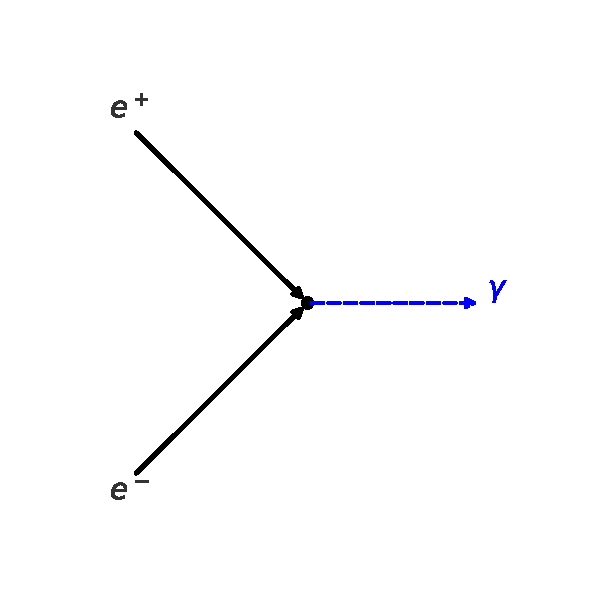
\includegraphics[height=8.5em]{bilder/qed-vertex.pdf} \quad \Rightarrow \quad -ie\gamma^\mu
	\]
	\caption{Wechselwirkungsterm}
\end{figure}
\vspace{0.5em}
\begin{tcolorbox}[didaktikbox, title=Vom Lagrange-Term zum Feynman-Vertex]
	\label{box:Vom Lagrange-Term zum Feynmann-Vertax}
	Die Kopplung in der Lagrangedichte erzeugt das QED-Vertex: ein Elektron, ein Positron, ein Photon treffen an einem Punkt zusammen. Diese Struktur bildet die Grundlage aller Diagramme in der QED.
\end{tcolorbox}
\index{Vertexfaktor $-ie\gamma^\mu$}

\subsubsection*{Eichinvarianz als Prinzip}\index{Eichinvarianz!lokal}\index{Eichtransformation}
\phantomsection
Die Form der QED-Lagrangedichte ist nicht beliebig gewählt. Sie ist das Resultat der Forderung, dass die Theorie \textbf{lokal eichinvariant} ist – also symmetrisch unter Transformationen der Form:
\[
\psi(x) \rightarrow e^{i\alpha(x)} \psi(x), \qquad A_\mu(x) \rightarrow A_\mu(x) - \frac{1}{e} \partial_\mu \alpha(x)
\]

Nur mit dieser Struktur bleibt die Theorie konsistent, relativistisch invariant und quantisierbar.\index{Quantisierbarkeit}

\subsubsection{Kopplung zwischen Elektronen und Photonen}\index{Kopplung!Elektronen–Photonen}\index{Lokale Eichinvarianz}

Die Wechselwirkung zwischen Elektron und Photon ergibt sich in der QED nicht „von außen“, sondern folgt aus einem fundamentalen Prinzip: der \textbf{lokalen Eichinvarianz}. Diese Symmetrie zwingt uns, das Photon als Kopplungspartner des Elektronenfeldes einzuführen.

\subsubsection*{Globale und lokale Phasentransformation}\index{Phasentransformation!global}\index{Phasentransformation!lokal}
\phantomsection
Ein Dirac-Feld $\psi$ ist invariant unter einer \textbf{globalen} Phasentransformation:
\[
\psi(x) \rightarrow e^{i\alpha} \psi(x)
\]
Die Lagrangedichte bleibt dabei unverändert – es handelt sich um eine Symmetrie.

Wenn man aber verlangt, dass $\alpha$ vom Ort abhängt, also
\[
\psi(x) \rightarrow e^{i\alpha(x)} \psi(x)
\]
spricht man von einer \textbf{lokalen Eichtransformation}. Diese zerstört die Invarianz der Lagrangedichte – es sei denn, man führt ein zusätzliches Feld $A_\mu(x)$ ein, das sich mittransformiert:
\[
A_\mu(x) \rightarrow A_\mu(x) - \frac{1}{e} \partial_\mu \alpha(x)
\]

\subsubsection*{Kovarianter Ableiter und minimaler Ersatz}\index{Kovarianter Ableiter}\index{Minimaler Ersatz}
\phantomsection
Damit die Theorie lokal eichinvariant bleibt, ersetzt man in der Dirac-Lagrangedichte die gewöhnliche Ableitung durch den \textbf{kovarianten Ableiter}:
\[
\partial_\mu \rightarrow D_\mu = \partial_\mu + ie A_\mu
\]

Dadurch entsteht automatisch ein Wechselwirkungsterm in der Lagrangedichte:
\[
\mathcal{L}_{\text{int}} = -e \, \bar{\psi} \gamma^\mu \psi A_\mu
\]

\vspace{0.5em}
\begin{tcolorbox}[mathebox, title=Kopplung aus Prinzip]
	\label{box:Kopplung aus Prinzip}
	Die Kopplung zwischen Elektron und Photon ist kein zusätzlicher Term, sondern folgt zwangsläufig aus der Forderung nach lokaler Eichinvarianz. Sie bestimmt die Form der Wechselwirkung eindeutig.
\end{tcolorbox}
\index{Viererstromdichte $\bar\psi\gamma^\mu\psi$}

\subsubsection*{Physikalische Bedeutung}\index{Physikalische Bedeutung!Kopplung}
\phantomsection
Der Ausdruck $\bar{\psi} \gamma^\mu \psi$ ist die \textbf{Viererstromdichte} des Elektronenfeldes. Der Term $A_\mu$ koppelt sich an diesen Strom – genau wie ein klassisches elektromagnetisches Feld an einen elektrischen Strom koppelt. Nur dass hier beide Größen quantisiert sind.\index{Strom!elektrisch}

\subsubsection*{Einfaches Bild: „Feld fühlt Feld“}\index{Anschauliches Bild}\index{Feld koppelt an Feld}
\phantomsection
Man kann sich den Prozess so vorstellen: Das Elektronenfeld „spürt“ das Photonfeld – weil seine Ableitung modifiziert wird. Wo früher nur der Gradient stand, steht nun ein Zusammenhang, der auch das Photon einbezieht.

\medskip
\begin{tcolorbox}[didaktikbox, title=Die Kraft entsteht aus dem Ableiter]
	\label{box:Die Kraft entsteht aus dem Ableiter}
	Die elektromagnetische Wechselwirkung entsteht in der QED dadurch, dass das Elektronenfeld auf den \emph{kovarianten} Ableiter reagiert. Dieser enthält das Photon – und damit ist die Kopplung erzeugt.
\end{tcolorbox}
\index{Kraft!Ursprung in $D_\mu$}

\subsubsection{Feynman-Regeln aus der Lagrangedichte}\index{Feynman-Regeln}\index{Störungstheorie}

Die Feynman-Diagramme sind keine bloßen Skizzen – sie folgen aus der Struktur der Lagrangedichte. Jeder Term der QED-Lagrangedichte hat eine klare Entsprechung in einem Baustein der Diagramme.

\subsubsection*{Grundprinzip: Störungsentwicklung}\index{Störungsentwicklung}\index{Feinstrukturkonstante $\alpha$}
\phantomsection
Da die Wechselwirkung in der QED schwach ist (die Feinstrukturkonstante $\alpha \approx 1/137$ ist klein), kann man physikalische Größen wie Übergangswahrscheinlichkeiten oder Streuamplituden als \textbf{Reihe in der Kopplungskonstanten} entwickeln. Jedes Glied dieser Reihe entspricht einem Feynman-Diagramm.\index{Übergangswahrscheinlichkeit}\index{Streuamplitude}

\subsubsection*{Elemente und ihre Bedeutung}\index{Propagator}\index{Vertex}\index{Impulsintegral}
\phantomsection
Aus der Lagrangedichte ergeben sich die folgenden Zuordnungen:

\vspace{0.5em}
\begin{tcolorbox}[mathebox, title=Feynman-Regeln der QED (vereinfacht)]
	\label{box:Feynman-Regeln der QED}
	\begin{itemize}
		\item \textbf{Elektronenlinie:} $\displaystyle \frac{i(\slashed{p} + m)}{p^2 - m^2 + i\varepsilon}$ (Dirac-Propagator)\index{Dirac-Propagator}
		\item \textbf{Photonenlinie:} $\displaystyle \frac{-ig^{\mu\nu}}{q^2 + i\varepsilon}$ (Photon-Propagator)\index{Photon-Propagator}
		\item \textbf{Vertex:} $-ie\gamma^\mu$\index{Vertexfaktor $-ie\gamma^\mu$}
		\item \textbf{Jede innere Linie:} Integration über Viererimpuls $d^4p$\index{Viererimpuls!Integration}
		\item \textbf{Gesamtdiagramm:} Produkt aller Faktoren, Integration über Schleifenimpulse\index{Schleifenimpuls}
	\end{itemize}
\end{tcolorbox}

\subsubsection*{Beispiel: Ein-Photon-Austausch}\index{Ein-Photon-Austausch}\index{Møller-Streuung}
\phantomsection
Die einfachste Anwendung ist die Møller-Streuung (Elektron-Elektron-Streuung über ein virtuelles Photon). Aus dem Vertex $-ie\gamma^\mu$ und den Propagatoren ergibt sich die Formel zur Streuamplitude. Die Berechnung folgt direkt aus den Feynman-Regeln – und liefert messbare Größen wie Wirkungsquerschnitte und Streuwinkel.\index{Wirkungsquerschnitt}

\subsubsection*{Ordnung der Diagramme}\index{Ordnung!in $e$}\index{Ordnung!in $\alpha$}\index{Loop-Korrekturen}
\phantomsection
Je mehr Vertices ein Diagramm enthält, desto höher ist seine Ordnung in $e$ bzw. in $\alpha = e^2 / (4\pi\hbar c)$. Niedrigere Ordnungen liefern die Hauptbeiträge, höhere Ordnungen die Korrekturen – etwa in Form von Schleifen (Loop-Korrekturen).

\medskip
\begin{tcolorbox}[didaktikbox, title=Warum die Regeln funktionieren]
	\label{box:Warum die Regeln funktionieren}
	Die Feynman-Regeln ergeben sich systematisch aus der QED-Lagrangedichte durch Anwendung der Störungstheorie. Sie sind also keine Ansammlung willkürlicher Anweisungen – sondern das direkte Resultat der Struktur der Theorie.
\end{tcolorbox}

\subsubsection*{Zusammenhang zur Messung}\index{Messung!Zusammenhang}\index{Theorie–Experiment}
\phantomsection
Jede beobachtbare Größe – Streuwinkel, Energieverteilung, g-Faktor-Korrektur – lässt sich mit Hilfe der Feynman-Regeln berechnen. Die Übereinstimmung mit dem Experiment macht die QED zur präzisesten Theorie der Physik.\index{Energieverteilung}

\subsubsection{Quantisierung des elektromagnetischen Feldes}\index{Quantisierung!elektromagnetisches Feld}\index{Photon!als Anregung}

In der klassischen Elektrodynamik ist das elektromagnetische Feld durch das Viererpotential $A^\mu(x)$ beschrieben. Doch solange dieses Feld nur klassische Gleichungen erfüllt (z.\,B. die Maxwell-Gleichungen), gibt es keine Photonen. Erst durch \textbf{Quantifizierung} wird aus dem Feld ein Quantensystem – und das Photon tritt als \emph{Anregung} dieses Feldes auf.\index{Maxwellsche Gleichungen}

\subsubsection*{Von der Welle zum Photon}\index{Moden!Quantisierung}\index{Fock-Raum}
\phantomsection
Das elektromagnetische Feld besteht aus unendlich vielen schwingenden Freiheitsgraden – ähnlich wie ein Gitarrensaite mit unendlich vielen möglichen Obertönen. Jeder Modus kann quantisiert werden. Dabei entsteht ein sogenannter \textbf{Fock-Raum}, in dem man Zustände wie
\[
\lvert 0 \rangle, \quad \lvert 1_{\vec{k}} \rangle, \quad \lvert 2_{\vec{k}} \rangle, \quad \dots
\]
beschreibt – also Zustände mit null, einem oder mehreren Photonen einer bestimmten Wellenzahl $\vec{k}$.\index{Vakuumzustand}\index{Photonenzahlzustand}

\subsubsection*{Das Photon als Anregung}\index{Photon!Quantenzustand}\index{Impuls $\hbar\vec{k}$}\index{Energie $\hbar\omega$}
\phantomsection
Ein Photon ist nichts anderes als ein Zustand mit einer einzigen Anregung des quantisierten Feldes $A^\mu(x)$ in einem bestimmten Modus. Diese Sichtweise ist grundlegend anders als die klassische Vorstellung einer Welle oder eines Teilchens.

\vspace{0.5em}
\begin{tcolorbox}[physikbox, title=Was ist ein Photon in der QED?]
	\label{box:Warum ist ein Photon in der QED}
	Ein Photon ist die einfachste Anregung des quantisierten elektromagnetischen Feldes. Es besitzt keine Ruhemasse, aber eine definierte Energie $E = \hbar \omega$ und einen Impuls $\vec{p} = \hbar \vec{k}$.
\end{tcolorbox}

\subsubsection*{Polarisation und Transversalität}\index{Polarisation}\index{Transversalität}\index{Helizität}
\phantomsection
Da das Photon masselos ist, hat es nur zwei physikalisch beobachtbare Polarisationszustände – nicht drei, wie bei einem massiven Spin-1-Teilchen. Das ist eine direkte Konsequenz der Eichinvarianz und der Transversalität der Welle:
\[
\vec{k} \cdot \vec{\epsilon} = 0
\]

Die QED behandelt dies korrekt durch den sogenannten \textbf{Gupta-Bleuler-Formalismus}\index{Gupta-Bleuler-Formalismus} oder über Feynman-Gaugen, bei denen auch unphysikalische Freiheitsgrade zunächst mitgeführt und später herausgerechnet werden.\index{Feynman-Gauß@Feynman-Gauge}

\subsubsection*{Eichsymmetrie und Freiheitsgrade}\index{Eichsymmetrie}\index{Freiheitsgrade}
\phantomsection
Die Eichsymmetrie erlaubt es, bestimmte Komponenten des Feldes $A^\mu$ durch Transformationen zu eliminieren. Physikalisch relevant bleiben nur die transversalen Anteile – und das sind genau die zwei Polarisationsrichtungen des Photons.

\medskip
\begin{tcolorbox}[didaktikbox, title=Warum hat das Photon keinen Spin-3-Zustand?]
	\label{box:Warum hat das Photon keinen Spin-3-Zustand}
	Ein massives Spin-1-Teilchen hätte drei Polarisationszustände. Aber weil das Photon masselos ist und das elektromagnetische Feld eichinvariant ist, bleiben nur zwei Zustände übrig. Diese entsprechen linearer oder zirkularer Polarisation.
\end{tcolorbox}

\index{Spin!Photon}\index{Zirkulare Polarisation}\index{Lineare Polarisation}

\subsubsection{Zusammenfassung}\index{Zusammenfassung!QED-Formalismus}
\addcontentsline{toc}{subsubsection}{Zusammenfassung}

Die Quantenelektrodynamik (QED) ist die quantisierte Feldtheorie der elektromagnetischen Wechselwirkung. Ihre mathematische Struktur basiert auf folgenden zentralen Elementen:

\begin{itemize}
	\item \textbf{Feldbeschreibung:} Elektronen und Positronen werden durch das Dirac-Feld $\psi(x)$ beschrieben, das Photon durch das Viererpotential $A^\mu(x)$.\index{Dirac-Feld}\index{Viererpotential}
	
	\item \textbf{Lagrangedichte:} Die QED-Lagrangedichte enthält drei Bestandteile:
	\begin{itemize}
		\item den freien Dirac-Term für das Elektronenfeld,\index{Dirac-Term}
		\item den freien Maxwell-Term für das Photonenfeld (Feldstärketensor $F_{\mu\nu}$),\index{Maxwell-Term}\index{Feldstärketensor $F_{\mu\nu}$}
		\item und den Kopplungsterm $-e \bar{\psi} \gamma^\mu \psi A_\mu$.\index{Kopplungsterm $-e\bar\psi\gamma^\mu\psi A_\mu$}
	\end{itemize}
	
	\item \textbf{Kopplung über Eichsymmetrie:} Die Form des Wechselwirkungsterms ergibt sich aus der Forderung lokaler Eichinvarianz. Sie erfordert die Einführung eines kovarianten Ableiters.\index{Kovarianter Ableiter}
	
	\item \textbf{Feynman-Regeln:} Aus der Lagrangedichte lassen sich die Bausteine der Feynman-Diagramme ableiten: Propagatoren, Vertices und Integrationsvorschriften.\index{Propagator}\index{Vertex}\index{Integrationsvorschriften}
	
	\item \textbf{Quantisierung des Photonenfeldes:} Durch Quantisierung des elektromagnetischen Feldes entstehen Photonen als Anregungen – mit zwei physikalischen Polarisationszuständen.\index{Quantisierung!Photonenfeld}\index{Polarisation!Photon}
	
\end{itemize}

Die QED ist in sich konsistent, relativistisch invariant, und stimmt in allen bisher getesteten Bereichen mit der experimentellen Realität überein.\index{Konsistenz}\index{Lorentzinvarianz} Die konkrete Berechnung physikalischer Größen erfolgt über Störungsreihen und Feynman-Diagramme – sie ist Thema des nächsten Kapitels.\index{Störungsreihen}

\subsection{Präzisionsexperimente}\index{Präzisionsexperimente}\index{Tests!QED}

In diesem Abschnitt soll die Rolle des Photons in modernen Hochpräzisionsexperimenten beleuchtet werden.\index{Photon!Rolle in Experimenten} Solche Experimente liefern nicht nur beeindruckende Bestätigungen der Quantenelektrodynamik (QED), sondern auch der speziellen Relativitätstheorie und fundamentaler Symmetrien der Natur.\index{Spezielle Relativitätstheorie}\index{Symmetrien!fundamental} Das Photon ist dabei nicht nur Objekt der Beobachtung, sondern oft auch das zentrale Werkzeug zur Untersuchung feinster physikalischer Effekte.\index{Photon!Messwerkzeug}

\subsubsection{Der anomale magnetische Moment des Elektrons}\index{Magnetisches Moment!anomales}\index{g-Faktor!Elektron}

Eines der am genauesten getesteten Ergebnisse der QED ist das sogenannte \emph{anomalous magnetic moment} des Elektrons, also die kleine Abweichung des $g$-Faktors von exakt 2:
\[
g_e \approx 2{,}00231930436...
\]
Diese Abweichung resultiert aus quantenfeldtheoretischen Korrekturen, insbesondere aus dem Austausch virtueller Photonen:\index{Korrekturen!quantenfeldtheoretisch}\index{Virtuelle Photonen!Schleifen}
\medskip
\begin{tcolorbox}[physikbox,title=Physikalische Bedeutung]
	\label{box:physikalische Bedeutung}
	Die Differenz von $g_e = 2$ zu dem experimentell gemessenen Wert wird durch Schleifenprozesse in Feynman-Diagrammen erklärt, bei denen virtuelle Photonen zwischen Elektron und sich selbst vermittelt werden. Die Übereinstimmung zwischen Theorie und Experiment ist ein Triumph der QED.
\end{tcolorbox}
\index{Triumph der QED}

\subsubsection{Lamb-Verschiebung}\index{Lamb-Shift}\index{Wasserstoff!Spektrum}

Ein weiteres spektakuläres Beispiel für die experimentelle Bestätigung der QED ist die \emph{Lamb-Verschiebung} der Energieniveaus im Wasserstoffatom. Der klassische Dirac-Formalismus sagt für das 2s- und 2p-Niveau dieselbe Energie voraus. Experimentell wurde jedoch eine winzige Energieverschiebung festgestellt:
\[
\Delta E_\text{Lamb} \approx \SI{1057}{\mega\hertz}
\]
\vspace{0.5em}
\begin{tcolorbox}[didaktikbox,title=Warum ist das wichtig?]
	\label{box:Warum ist wichtig}
	Die Lamb-Verschiebung zeigt, dass der leere Raum – das Quantenvakuum – nicht „leer“ ist. Virtuelle Photonen bewirken Fluktuationen, die die Energieniveaus beeinflussen.
\end{tcolorbox}
\index{Quantenvakuum}\index{Vakuumfluktuationen}
\subsubsection{Spektroskopie und Konstanzmessungen}\index{Spektroskopie}\index{Naturkonstanten!Messungen}\index{Frequenzkamm}\index{Atomuhr}

Photonenbasierte Hochpräzisions-Spektroskopie liefert auch genaueste Messungen fundamentaler Naturkonstanten wie:

\begin{itemize}
	\item der Feinstrukturkonstante $\alpha$\index{Feinstrukturkonstante $\alpha$}
	\item der Planck-Konstante $h$\index{Planck-Konstante $h$}
	\item der Lichtgeschwindigkeit $c$ (heute fest definiert)\index{Lichtgeschwindigkeit $c$}
\end{itemize}

Diese Messungen stützen sich auf Lasertechnologie, Frequenzkämme und Atomuhren – allesamt photonengebundene Techniken.\index{Laser}\index{Photonentechniken}

\subsubsection{Tests fundamentaler Symmetrien}\index{Symmetrien!Tests}\index{CPT-Invarianz}\index{Lorentz-Invarianz}

Experimente mit Photonen tragen dazu bei, fundamentale Symmetrien zu testen:

\begin{itemize}
	\item \textbf{CPT-Invarianz:} Präzisionsmessungen am Antiwasserstoff vergleichen Spektrallinien mit gewöhnlichem Wasserstoff.\index{Antiwasserstoff}
	\item \textbf{Lorentz-Invarianz:} Richtungsabhängigkeiten der Lichtgeschwindigkeit werden mit resonatorgestützten Lasersystemen überprüft.\index{Resonator!optisch}
\end{itemize}
\vspace{0.5em}
\begin{tcolorbox}[hypobox, title={Was wäre, wenn Licht nicht isotrop wäre?}]
	\label{box:was wäre nicht isotop}
	
	Würde man eine Richtungsabhängigkeit der Lichtgeschwindigkeit messen, wäre das ein Hinweis auf eine fundamentale Verletzung der Lorentz-Symmetrie – mit drastischen Folgen für die Relativitätstheorie und unser physikalisches Weltbild.
\end{tcolorbox}
\index{Isotropie des Lichts}\index{Lorentz-Symmetrie!Verletzung}

\subsubsection{Zusammenfassung}\index{Zusammenfassung!Präzisionsexperimente}

Präzisionsexperimente sind eine der stärksten Säulen zur Überprüfung unserer physikalischen Theorien. Sie zeigen, wie weitreichend und verlässlich das Konzept des Photons in der modernen Physik verankert ist. Besonders die Quantenelektrodynamik beweist hier ihre beispiellose Genauigkeit – und mit ihr die zentrale Rolle des Photons als Austauschteilchen und Informationsträger.\index{Informationsträger!Photon}

\subsection{Fazit}
% Zusammenfassung der Rolle des Photons in der QED, Übergang zu Kapitel VI

In Kapitel~V haben wir das Photon als zentrales Vermittlungsteilchen der elektromagnetischen Wechselwirkung im Rahmen der Quantenelektrodynamik (QED) kennengelernt.\index{Vermittlungsteilchen} Beginnend mit dem Übergang vom klassischen Lichtquant zum quantisierten Feld wurde deutlich, wie tief die Struktur der QED mit dem Photon verknüpft ist. 

Wir haben gesehen:
\begin{itemize}
	\item wie sich das Photon mathematisch als Vektorfeld mit Eichfreiheit beschreiben lässt,\index{Vektorfeld!Photon}\index{Eichfreiheit}
	\item wie virtuelle Photonen in Feynman-Diagrammen die Wechselwirkung zwischen geladenen Teilchen vermitteln,\index{Virtuelle Photonen!Vermittlung}
	\item wie der QED-Formalismus über Eichsymmetrie, Lagrangedichte und Störungstheorie aufgebaut ist,\index{QED!Aufbau}\index{Störungstheorie}
	\item und wie Präzisionsexperimente – vom $g$-Faktor bis zur Lamb-Verschiebung – die Theorie mit beispielloser Genauigkeit bestätigen.\index{Bestätigung!experimentell}
\end{itemize}

Die Quantenelektrodynamik zählt zu den erfolgreichsten Theorien der Physik. Sie liefert nicht nur präzise Vorhersagen, sondern auch ein tiefes Verständnis der Rolle des Photons – als masseloses, aber wirkungsmächtiges Quantenobjekt.\index{Quantenobjekt!Photon} 

\medskip
\begin{tcolorbox}[hinweisbox,title=Ausblick auf Kapitel VI]
	\label{box:Ausblick auf Kapitel 6}
	Im nächsten Kapitel betrachten wir Anwendungen des Photons in Praxis und Forschung – von der Lasertechnologie über Quantensensoren bis zur Rolle in der modernen Kommunikation.
\end{tcolorbox}
\index{Lasertechnologie}\index{Quantensensorik}\index{Quantenkommunikation}
